\chapter{The Importance of Data Structures}
\label{cha:ChartParsing}

Remember that we analyze parsers as the combination of three components: a parsing schema, a control structure, and a data structure.
While parsing schema and certain aspects of the control structure have occupied a lot of our attention, we haven't talked much about data structures so far.
Our psycholinguistic evaluations used a prefix tree as a representation of the parse space and how it might be explored by the parser, but we did not assume that the parser actually uses a prefix tree to store information.
However, we did propose that the control structure might operate on a priority queue as an encoding of which parse to explore next.
A priority queue is a form of data structure as it holds the parse items inferred by the parser.
But it cannot be the full data structure: since items are frequently removed from the queue, it does not provide a permanent record of the actual parse.
One option would be to build and store each individual parse trees in parallel with the parse, but as we will see this is too inefficient even for computers, whose working memory vastly outstrips that of humans.
It is about time, then, that we take a more careful look at data structures and the parsers that make use of them. 

\section{Why Data Structures Matter}

Recall from Chap.~\ref{cha:BigPicture} that we distinguish between parsers and recognizers.
A recognizer only has to determine for a given sentence whether it is well-formed, whereas a parser also has to find the right tree structures.

One might think that data structures are less of a concern for recognizers.
Any one of our parsing schema coupled with a priority queue yields a working recognizer.
The fact that the priority queue does not store parse items after they have been used in an inference rule is irrelevant since the only thing that matters is whether the priority queue contains a parse item that is a goal for the input sentence.
As soon as this condition is satisfied, the recognizer can stop and declare the input sentence well-formed.

Even for a recognizer, though, there are downsides to not storing previous items.
Most problematically, the recognizer may accidentally enter a loop if there are two items $I$ and $J$ such that each one can be inferred from the other.
If neither $I$ nor $J$ allow the sentence to be recognized, and the control structure is designed in such a way that $I$ and $J$ are preferred to other items that would eventually lead to successful recognition of the input, then the recognizer will try the $I$-route and the $J$-route over and over again.
In less severe cases the recognizer does not enter a loop but ends up exploring partial parses that have already turned out to be failures at an earlier point.
%
\begin{examplebox}[Needlees Reexploration of Failed Partial Parses]
    The parse history of the recursive descent parser\slash recognizer for the garden path sentence \emph{the horse raced past the barn} includes several cases of redundancy.
    %
    \begin{center}
        \footnotesize
        \begin{tikzpicture}[%
            level 1+/.style = { level distance = 2em },
            level 5/.style = { sibling distance= -5em },
            level 7/.style = { sibling distance= -5em },
            level 8/.style = { sibling distance= -10em }
            ]
            \Tree
                [.{[0,\psep S]}
                    [.{[0,\psep NP VP]}
                        [.{[0,\psep Det N VP]}
                            [.{[0, \psep the N VP]}
                                [.{[1,\psep N VP]}
                                    [.{[1,\psep horse VP]}
                                        [.{[2,\psep VP]}
                                            [.{[2,\psep V PP]}
                                                [.{[2,\psep raced PP]}
                                                    [.{[3,\psep PP]}
                                                        [.{[3,\psep P NP]}
                                                            [.{[3,\psep past NP]}
                                                                [.{[4,\psep NP]}
                                                                    [.{[4,\psep Det N]}
                                                                        [.{[4,\psep the N]}
                                                                            [.{[5,\psep N]}
                                                                                [.{[5,\psep barn]}
                                                                                    {[6,\psep]}
                                                                                ]
                                                                                {[5,\psep horse]}
                                                                            ]
                                                                        ]
                                                                    ]
                                                                    [.{[4,\psep Det N VP$_\mathit{rel}$]}
                                                                        [.{[4,\psep the N VP$_\mathit{rel}$]}
                                                                            [.{[5,\psep N VP$_\mathit{rel}$]}
                                                                                [.{[5,\psep barn VP$_\mathit{rel}$]}
                                                                                    [.{[6,\psep VP$_\mathit{rel}$]}
                                                                                        [.{[6,\psep V$_\mathit{rel}$ PP]}
                                                                                            {[6,\psep fell PP]}
                                                                                        ]
                                                                                    ]
                                                                                ]
                                                                                {[5,\psep horse VP$_\mathit{rel}$]}
                                                                            ]
                                                                        ]
                                                                    ]
                                                                ]
                                                            ]
                                                        ]
                                                    ]
                                                ]
                                                {[2,\psep fell PP]}
                                            ]
                                            [.{[2,\psep V]}
                                                {[2,\psep raced]}
                                                {[2,\psep fell]}
                                            ]
                                        ]
                                    ]
                                {[1,\psep barn VP]}
                                ]
                            ]
                        ]
                        [.{[0,\psep Det N VP$_\mathit{rel}$ VP]}
                            [.{[0,\psep the N VP$_\mathit{rel}$ VP]}
                                [.{[1,\psep N VP$_\mathit{rel}$ VP]}
                                    {[1,\psep barn VP$_\mathit{rel}$ VP]}
                                    [.{[1,\psep horse VP$_\mathit{rel}$ VP]}
                                        [.{[2,\psep VP$_\mathit{rel}$ VP]}
                                            [.{[2,\psep V$_\mathit{rel}$ PP VP]}
                                                [.{[3,\psep raced PP VP]}
                                                    [.{[4,\psep PP VP]}
                                                        [.{[4,\psep P NP VP]}
                                                            [.{[4,\psep past NP VP]}
                                                                [.{[5,\psep NP VP]}
                                                                    [.{[5,\psep Det N VP]}
                                                                        [.{[5,\psep the N VP]}
                                                                            [.{[6,\psep N VP]$_{10}$}
                                                                                [.{[6,\psep barn VP]}
                                                                                    [.{[7,\psep VP]}
                                                                                        [.{[7,\psep V]$_{13}$}
                                                                                            [.{[7,\psep fell]}
                                                                                                {[7,\psep]}
                                                                                            ]
                                                                                        ]
                                                                                    ]
                                                                                ]
                                                                            ]
                                                                        ]
                                                                    ]
                                                                ]
                                                            ]
                                                        ]
                                                    ]
                                                ]
                                            ]
                                        ]
                                    ]
                                ]
                            ]
                        ]
                    ]
                ]
        \end{tikzpicture}
    \end{center}
    %
    After the failed exploration of the left-most branch, the recognizer backtracks and uses [5,\psep N] to infer [5,\psep horse] instead of [5,\psep barn].
    Since the word at position 5 is \emph{horse}, not \emph{barn}, this branch obviously fails, too.
    What more, we can infer that every  parse item of the form [5,\psep horse $\gamma$] will lead to failure.
    Yet the parser attempts the very same thing in the next branch with [5,\psep horse VP$_\mathit{rel}$].
    Later on, a similar instance of redundancy arises when [1, \psep barn VP$_\mathit{rel}$ VP] is conjectured even though [1,\psep barn VP] has already failed.
\end{examplebox}
%
\noindent
If parse items are discarded immediately after being used in an inference rule, the recognizer also loses the ability to recycle successful partial parses.
%
\begin{examplebox}[Needless Reexploration of Successful Partial Parses]
    Suppose the sentence \emph{Red Riding Hood met the big, bad wolf yesterday} is to be recognized using the following grammar:
    %
    \begin{center}
        \begin{tabular}{rcl@{\hspace{2em}}rcl}
            S    & \rewrite & NP VP
                 & 
            PN   & \rewrite & Red Riding Hood
            \\
            NP   & \rewrite & PN | Det N | Det AP N
                 & 
            Det  & \rewrite & the
            \\
            AP   & \rewrite & Adj | Adj AP
                 & 
            N    & \rewrite & wolf
            \\
            VP   & \rewrite & Vi | Vt NP | VP AdvP
                 & 
            Adj  & \rewrite & bad | big
            \\
            AdvP & \rewrite & Adv
                 & 
            Adv  & \rewrite & yesterday
            \\
                 &          &                      & 
            Vi   & \rewrite & left
            \\
                 &          &                      & 
            Vt   & \rewrite & left | met
        \end{tabular}
    \end{center}
    %
    Assume furthermore that the linear order of disjunctive right-hand sides encodes their priority in the control structure.
    Then a recursive descent recognizer will first go through the options below rewriting VP as Vi or Vt NP, neither of which produces a goal item.
    %
    \begin{center}
        \footnotesize
        \begin{tikzpicture}[
            level 1+/.style = { level distance = 2em }
            ]
            \Tree
                [.{[0,\psep S]}
                    [.{[0,\psep NP VP]}
                        [.{[0,\psep PN VP]}
                            [.{[0,\psep RRH VP]}
                                [.{[1,\psep VP]}
                                    [.{[1,\psep Vi]}
                                        [.{[1, \psep left]}
                                        ]
                                    ]
                                    [.{[1,\psep Vt NP]}
                                        [.{[1,\psep left NP]}
                                        ]
                                        [.{[1,\psep met NP]}
                                            [.{[2,\psep NP]}
                                                [.{[2,\psep PN]}
                                                    [.{[2,\psep RRH]}
                                                    ]
                                                ]
                                                [.{[2,\psep Det N]}
                                                    [.{[2,\psep the N]}
                                                        [.{[4,\psep N]}
                                                            [.{[4,\psep wolf]}
                                                            ]
                                                        ]
                                                    ]
                                                ]
                                                [.{[2,\psep Det AP N]}
                                                    [.{[2,\psep the AP N]}
                                                        [.{[3,\psep AP N]}
                                                            [.{[3,\psep Adj N]}
                                                                [.{[3,\psep bad N]}
                                                                ]
                                                                [.{[3,\psep big N]}
                                                                    [.{[5,\psep N]}
                                                                        [.{[5,\psep wolf]}
                                                                        ]
                                                                    ]
                                                                ]
                                                            ]
                                                            [.{[3,\psep Adj AP N]}
                                                                [.{[3,\psep bad AP N]}
                                                                ]
                                                                [.{[3,\psep big AP N]}
                                                                    [.{[4,\psep AP N]}
                                                                        [.{[4,\psep Adj N]}
                                                                            [.{[4,\psep bad N]}
                                                                                [.{[5,\psep N]}
                                                                                    [.{[5,\psep wolf]}
                                                                                        [.{[6,\psep]}
                                                                                        ]
                                                                                    ]
                                                                                ]
                                                                            ]
                                                                        ]
                                                                    ]
                                                                ]
                                                            ]
                                                        ]
                                                    ]
                                                ]
                                            ]
                                        ]
                                    ]
                                ]
                            ]
                        ]
                    ]
                ]
        \end{tikzpicture}
    \end{center}
    %
    As before we see that the recognizer repeats inferences that have already failed before, e.g.\ [1,\psep left NP] after [1,\psep left].
    A bigger problem is revealed once we look at the parse history after the recognizer correctly infers [1,\psep VP AdvP] from [1,\psep VP].
    %
    \begin{center}
        \footnotesize
        \begin{tikzpicture}[
            level 1+/.style = { level distance = 2em }
            ]
            \Tree
                [.{[1,\psep VP AdvP]}
                    [.{[1,\psep VP AdvP]}
                        [.{[1,\psep Vi AdvP]}
                            [.{[1, \psep left AdvP]}
                            ]
                        ]
                        [.{[1,\psep Vt NP AdvP]}
                            [.{[1,\psep left NP AdvP]}
                            ]
                            [.{[1,\psep met NP AdvP]}
                                [.{[2,\psep NP AdvP]}
                                    [.{[2,\psep PN AdvP]}
                                        [.{[2,\psep RRH AdvP]}
                                        ]
                                    ]
                                    [.{[2,\psep Det N AdvP]}
                                        [.{[2,\psep the N AdvP]}
                                            [.{[3,\psep N AdvP]}
                                                [.{[3,\psep wolf AdvP]}
                                                ]
                                            ]
                                        ]
                                        [.\node(link-top){\phantom{[]}};
                                        ]
                                    ]
                                ]
                            ]
                        ]
                    ]
                ]

            \begin{scope}[yshift=-22em]
                \Tree
                    [.\node(link-bottom){[3,\psep Det AP N AdvP]};
                        [.{[2,\psep the AP N AdvP]}
                            [.{[3,\psep AP N AdvP]}
                                [.{[3,\psep Adj N AdvP]}
                                    [.{[3,\psep bad N AdvP]}
                                    ]
                                    [.{[3,\psep big N AdvP]}
                                        [.{[4,\psep N AdvP]}
                                            [.{[4,\psep wolf AdvP]}
                                            ]
                                        ]
                                    ]
                                ]
                                [.{[3,\psep Adj AP N AdvP]}
                                    [.{[3,\psep bad AP N AdvP]}
                                    ]
                                    [.{[3,\psep big AP N AdvP]}
                                        [.{[4,\psep AP N AdvP]}
                                            [.{[4,\psep Adj N AdvP]}
                                                [.{[4,\psep bad N AdvP]}
                                                    [.{[5,\psep N AdvP]}
                                                        [.{[5,\psep wolf AdvP]}
                                                            [.{[6,\psep AdvP]}
                                                                [.{[6,\psep Adv]}
                                                                    [.{[6,\psep yesterday]}
                                                                        [.{[7,\psep]}
                                                                        ]
                                                                    ]
                                                                ]
                                                            ]
                                                        ]
                                                    ]
                                                ]
                                            ]
                                        ]
                                    ]
                                ]
                            ]
                        ]
                    ]
            \end{scope}

            \draw (link-top.north) .. controls +(310:14em) and +(55:6em) .. (link-bottom.north);    
        \end{tikzpicture}
        %
    \end{center}
    %
    This subtree of the parse history is virtually isomorphic to the one rooted in [1,\psep VP] --- the only difference is that the last branch expands the AdvP and finally reaches a goal item.
    What this means is that the recognizer does not reuse any of the information it collected on its first attempt to build the VP\@.
    It has to verify again that the verb is \emph{met}, and it builds the NP for \emph{big, bad wolf} from scratch even though it had already been correctly recognized in the [1,\psep VP] subtree.
\end{examplebox}
%
This shows that even for recognizers a good data structure is essential to
%
\begin{itemize}
    \item detect and avoid loops,
    \item skip inferences that have failed before,
    \item reuse successful inferences.
\end{itemize}
%
Once a useful data structure is in place, using it as a record of parse trees and thereby expanding the recognizer to a parser is just a minor step.

\section{Chart Parsing}

\section{CKY}

\subsection{Intuition}

The Cock-Younger-Kasami parser --- usually abbreviated CYK or CKY --- is not only the best-known chart parsing algorithm, it is probably also the most popular parser in computational linguistics.
That's probably due to its high efficiency coupled with its conceptual simplicity.
The idea behind the CKY parser is indeed very simple: we read in the entire input string and then carry out all possible bottom-up reductions in parallel.
In a certain sense, the CKY parser behaves like a shift-reduce parser where \textsc{i}) we always apply shift until we have reached the end of the string, and \textsc{ii}) parse items can participate in multiple reduction steps.

The CKY parser is usually specified in the format of a chart parser.
Suppose we have the input string \emph{the anvil hit the duck on the head}.
Our first step is to draw a matrix that has as many columns and rows as there are words in the input.
We will only use the fields above the diagonal, so the others are shaded out.
It will be convenient to refer to individual cells by their address $(i,j)$, where $i$ is the row number and $j$ the column number.
The idea is that each cell $(i,j)$ represents the substring of the input spanning from position $i$ to $j$.
%
\begin{center}
    \begin{tabular}{r | C{3em} C{3em} C{3em} C{3em} C{3em} C{3em} C{3em} C{3em} |}
          & 1 & 2 & 3 & 4 & 5 & 6 & 7 & 8\\
          \hline
        0 & & & & & & & & \\
        1 & \cellcolor{gray!25} & & & & & & & \\
        2 & \cellcolor{gray!25} & \cellcolor{gray!25} & & & & & & \\
        3 & \cellcolor{gray!25} & \cellcolor{gray!25} & \cellcolor{gray!25} & & & & & \\
        4 & \cellcolor{gray!25} & \cellcolor{gray!25} & \cellcolor{gray!25} & \cellcolor{gray!25} & & & & \\
        5 & \cellcolor{gray!25} & \cellcolor{gray!25} & \cellcolor{gray!25} & \cellcolor{gray!25} & \cellcolor{gray!25} & & & \\
        6 & \cellcolor{gray!25} & \cellcolor{gray!25} & \cellcolor{gray!25} & \cellcolor{gray!25} & \cellcolor{gray!25} & \cellcolor{gray!25} & & \\
        7 & \cellcolor{gray!25} & \cellcolor{gray!25} & \cellcolor{gray!25} & \cellcolor{gray!25} & \cellcolor{gray!25} & \cellcolor{gray!25} & \cellcolor{gray!25} & \\
        \hline
          & the & anvil & hit & the & duck & on & the & head\\
    \end{tabular}
\end{center}
%
For each word $w_i$ in the input, we enter all possible parts of speech in the cell $(i,i+1)$.
%
\begin{center}
    \begin{tabular}{r | C{3em} C{3em} C{3em} C{3em} C{3em} C{3em} C{3em} C{3em} |}
          & 1 & 2 & 3 & 4 & 5 & 6 & 7 & 8\\
          \hline
        0 & Det & & & & & & & \\
        1 & \cellcolor{gray!25} & N & & & & & & \\
        2 & \cellcolor{gray!25} & \cellcolor{gray!25} & N,V & & & & & \\
        3 & \cellcolor{gray!25} & \cellcolor{gray!25} & \cellcolor{gray!25} & Det & & & & \\
        4 & \cellcolor{gray!25} & \cellcolor{gray!25} & \cellcolor{gray!25} & \cellcolor{gray!25} & N,V & & & \\
        5 & \cellcolor{gray!25} & \cellcolor{gray!25} & \cellcolor{gray!25} & \cellcolor{gray!25} & \cellcolor{gray!25} & P & & \\
        6 & \cellcolor{gray!25} & \cellcolor{gray!25} & \cellcolor{gray!25} & \cellcolor{gray!25} & \cellcolor{gray!25} & \cellcolor{gray!25} & Det & \\
        7 & \cellcolor{gray!25} & \cellcolor{gray!25} & \cellcolor{gray!25} & \cellcolor{gray!25} & \cellcolor{gray!25} & \cellcolor{gray!25} & \cellcolor{gray!25} & N\\
        \hline
          & the & anvil & hit & the & duck & on & the & head\\
    \end{tabular}
\end{center}
%
In order to fill in the remaining cells, we use the following algorithm: if cell $(i,j)$ contains category $B$ and cell $(j,k)$ contains category $C$ and $A \rewrite B C$ is a rewrite rule of the grammar, then enter $A$ in cell $(i,k)$.
%
\begin{center}
    \begin{tabular}{r | C{3em} C{3em} C{3em} C{3em} C{3em} C{3em} C{3em} C{3em} |}
          & 1 & 2 & 3 & 4 & 5 & 6 & 7 & 8\\
          \hline
        0 & Det & NP & & & S & & & S\\
        1 & \cellcolor{gray!25} & N & & & & & & \\
        2 & \cellcolor{gray!25} & \cellcolor{gray!25} & N,V & & VP & & & VP\\
        3 & \cellcolor{gray!25} & \cellcolor{gray!25} & \cellcolor{gray!25} & Det & NP & & & NP\\
        4 & \cellcolor{gray!25} & \cellcolor{gray!25} & \cellcolor{gray!25} & \cellcolor{gray!25} & N,V & & & \\
        5 & \cellcolor{gray!25} & \cellcolor{gray!25} & \cellcolor{gray!25} & \cellcolor{gray!25} & \cellcolor{gray!25} & P & & PP\\
        6 & \cellcolor{gray!25} & \cellcolor{gray!25} & \cellcolor{gray!25} & \cellcolor{gray!25} & \cellcolor{gray!25} & \cellcolor{gray!25} & Det & NP\\
        7 & \cellcolor{gray!25} & \cellcolor{gray!25} & \cellcolor{gray!25} & \cellcolor{gray!25} & \cellcolor{gray!25} & \cellcolor{gray!25} & \cellcolor{gray!25} & N\\
        \hline
          & the & anvil & hit & the & duck & on & the & head\\
    \end{tabular}
\end{center}
%
The input is well-formed iff the top-right cell contains the start category S\@.
In other words, there is a constituent labeled S that spans the entire input string.

With a chart like the one above, the CKY algorithm is just a recognizer as it is not always obvious how specific cell values were derived from others.
For instance, the cell $(3,5)$ contains the value NP, but there is no indication whether this NP consists of Det N or Det V\@.
Similarly, the VP in cell $(2,8)$ could be the result of combining either the V in $(2,3)$ with the NP in $(3,8)$ or the VP in $(2,5)$ with the PP in $(5,8)$.
These alternatives correspond to very different structures: one where the PP is an NP adjunct, and another one with the PP as a VP adjunct.

In order to turn CKY from a recognizer into a parser, we have to modify the cell values such that each category comes with backpointers that indicate which other categories were used in the reduction.
We can represent this pictorially by adding arrows to the chart.
%
\begin{center}
    \begin{tabular}{r | C{3em} C{3em} C{3em} C{3em} C{3em} C{3em} C{3em} C{3em} |}
          & 1 & 2 & 3 & 4 & 5 & 6 & 7 & 8\\
          \hline
        0 & \tikz[remember picture](the){Det}; & NP & & & S & & & S\\
        1 & \cellcolor{gray!25} & N & & & & & & \\
        2 & \cellcolor{gray!25} & \cellcolor{gray!25} & N,V & & VP & & & VP\\
        3 & \cellcolor{gray!25} & \cellcolor{gray!25} & \cellcolor{gray!25} & Det & NP & & & NP\\
        4 & \cellcolor{gray!25} & \cellcolor{gray!25} & \cellcolor{gray!25} & \cellcolor{gray!25} & N,V & & & \\
        5 & \cellcolor{gray!25} & \cellcolor{gray!25} & \cellcolor{gray!25} & \cellcolor{gray!25} & \cellcolor{gray!25} & P & & PP\\
        6 & \cellcolor{gray!25} & \cellcolor{gray!25} & \cellcolor{gray!25} & \cellcolor{gray!25} & \cellcolor{gray!25} & \cellcolor{gray!25} & Det & NP\\
        7 & \cellcolor{gray!25} & \cellcolor{gray!25} & \cellcolor{gray!25} & \cellcolor{gray!25} & \cellcolor{gray!25} & \cellcolor{gray!25} & \cellcolor{gray!25} & N\\
        \hline
          & the & anvil & hit & the & duck & on & the & head\\
    \end{tabular}
\end{center}

\subsection{Formal Specification}

Axiom: $[i,a,i+1]$ for each $a = w_i$
Goal: $[0,S,n]$

\begin{prooftree}
    \AxiomC{$[i, B, j]$}
    \AxiomC{$[j, C, k]$}
    \LeftLabel{\textbf{Reduce}\qquad}
    \BinaryInfC{$[i, A, k]$}
\end{prooftree}


\section{Earley}

\subsection{Intuition}

\subsection{Formal Specification}
Axiom: $[0, S' \rewrite \psep S,0]$
Goal: $[0, S' \rewrite S \psep,0]$

\begin{prooftree}
    \AxiomC{$[i, A \rewrite \alpha \psep a \beta,j]$}
    \LeftLabel{\textbf{Scan}\qquad}
    \RightLabel{$a = w_{i}$}
    \UnaryInfC{$[i, A \rewrite \alpha a \psep \beta, j+1]$}
\end{prooftree}

\begin{prooftree}
    \AxiomC{$[i, A \rewrite \alpha \psep B \beta,j]$}
    \LeftLabel{\textbf{Predict}\qquad}
    \RightLabel{$B \rewrite \gamma \in R$}
    \UnaryInfC{$[j, B \rewrite \psep \gamma, j]$}
\end{prooftree}

\begin{prooftree}
    \AxiomC{$[i, A \rewrite \alpha \psep B \beta,j]$}
    \AxiomC{$[j, B \rewrite \gamma \psep,k]$}
    \LeftLabel{\textbf{Complete}\qquad}
    \BinaryInfC{$[i, A \rewrite \alpha B \psep \beta,k]$}
\end{prooftree}

\subsection{Left Recursion is Unproblematic}

\subsection{Relation to Left Corner Parsing}
